\documentclass[11pt]{article}
\pdfpxdimen=1in
\divide\pdfpxdimen by 300
 
\usepackage[latin1]{inputenc}
\usepackage[T1]{fontenc}
\usepackage[english]{babel}
\usepackage{mathtools, bm}
\usepackage{amssymb, bm}
\usepackage{float}

\usepackage{caption} % to center captions
\usepackage{subcaption} % subcaption for figures side by side
\usepackage[table,xcdraw]{xcolor}  % to put color in tables

\usepackage[parfill]{parskip}
\usepackage{graphicx}
\usepackage{hyperref}
\usepackage[top=0.5in, bottom=0.5in, left=1in, right=1in]{geometry}
\usepackage{listings}

\renewcommand\thesection{\Roman{section}} % Section starting with I, II, ...
\renewcommand\thesubsection{\thesection.\Alph{subsection}} % Subsection starting with A, B, ...

\renewcommand\thefigure{\thesubsection.\arabic{figure}}

\newcommand{\horrule}[1]{\rule{\linewidth}{#1}} % Create horizontal rule command with 1 argument of height

\numberwithin{figure}{section} % to have per-section figure numbering

\title{	
\normalfont \normalsize 
\textsc{Master MVA \\
Object Recognition and Computer Vision} \\ [20pt]
\horrule{0.5pt} \\[0.2cm] % Thin top horizontal rule
\textbf{Assignment 1}: Instance Level Recognition \\
\horrule{2pt} \\[0.3cm] % Thick bottom horizontal rule
}

\author{Victor Busa \\
   \texttt{victor.busa@ens-paris-saclay.fr}}

\date{\normalsize\today}

\begin{document}

\maketitle

\section{Sparse features for matching specific objects in images}
\subsection{SIFT features detections}
\paragraph{}\textbf{1.} It is important to obtain similarity co-variant features for matching because, in real life, images undergo various transformations (scaling, rotation, translation, shear, lighting, ...)  depending on the point of view from which the picture was taken. Hence, we need a model that does not depend upon these transformations.

\paragraph{}\textbf{2.} 
\begin{figure}[!h] 
  \centering
	\includegraphics[scale=0.8]{SIFT_features.eps}
  \caption{detected features for three different values of the peakThreshold}
\end{figure}

\paragraph{}\textbf{3.} The density of detections across images change with the \textit{peakThreshold}. Indeed, the \textit{peakThreshold} parameter allows rejecting the potential key-points locations found if the intensity of those points is less then the \textit{peakThreshold} value. Hence, the matching won't work as well when the two images have different intensity (luminosity). We can fix the drawback of this technique by preprocessing the images in order to bring them to the same intensity (luminosity).

\begin{figure}[!h] 
  \centering
	\captionsetup{justification=centering}
	\includegraphics[scale=0.4]{intensity.eps}
  \caption{The number of detected features depends upon the intensity (luminosity) of the image. here \textbf{peakThreshold = 0.007}}
\end{figure}

\subsection{SIFT features descriptors and matching between images}
\paragraph{}\textbf{1.} The fact that the descriptors are computed over a much larger region than the detection is a good idea in the sense that the matching will occur on a broader space and hence the detection would likely be more accurate.

\begin{figure}[H]
\centering
\begin{minipage}{.5\textwidth}
  \centering
  \includegraphics[scale=1]{features_descriptors.eps}
  \captionof{figure}{SIFT descriptors}
  \label{fig:test1}
\end{minipage}%
\begin{minipage}{.5\textwidth}
  \centering
  \includegraphics[scale=0.4]{nn_matches.eps}
  \captionof{figure}{Nearest neighbour matches}
  \label{fig:test2}
\end{minipage}
\end{figure}

\paragraph{}\textbf{2.} As we can see in Figure I.2, mismatches are lighting dependent. Actually, SIFT doesn't work well when there are either a large illumination change or nonrigid deformations. To reduce the amount of mismatch, one can use a cluster of at least 3 features that agree with the geometrical position of an object. These clusters are more likely to be correct than if we only focus on individual feature matches.

\begin{figure}[H]
  \centering
	\includegraphics[scale=0.7]{mismatch_intensity_dependents.eps}
  \caption{Effect of lighting on the SIFT descriptors}
\end{figure}


\begin{figure}[H] 
  \centering
	\captionsetup{justification=centering}
	\includegraphics[scale=0.7]{secondNN.eps}
  \caption{Effect of the second nearest neighbor threshold on the number of correct and incorrect matches}
\end{figure}

\subsection{Improving SIFT matching using Lowe\'s second nearest neighbor test}

\paragraph{}\textbf{1.} We can considerably reduce the number of mismatches while discarding very few correct matches by using the second nearest neighbor test. The idea behind this technique relies on the fact that:
\begin{itemize}
\item correct matches need to have the first nearest neighbor closer than the closest incorrect match (second nearest neighbor)
\item false matches will have the first and second nearest neighbor within a similar distance. Hence false matches will have a ratio: $\frac{1NN}{2NN} \approx 1$
\end{itemize}

We can see in Figure I.6 that the higher the \textit{nnThreshold} is, the more matches we have. Also, a good trade-off is around 0.8. Above 0.8 we will keep too many mismatches. Below 0.8 we will have too few matches.

\subsection{Improving SIFT matching using a geometric transformation}

\paragraph{}\textbf{1.} TO DO

\paragraph{}\textbf{2.} For each tentative correspondence, we compute the similarity transformation. Then we apply the same step as in the RANSAC algorithm. At the end, after testing several affine transformations, we select the one with the highest count of inliers. \newline
We can see in Figure I.7 that there are fewer matches than when using the second nearest neighbor test with a threshold of 0.8. Yet, we can clearly see that these matches are very accurate (we can quickly see that all the lines between matches are parallel).


\begin{figure}[!h] 
  \centering
	\includegraphics[scale=0.5]{geometric_verification.eps}
  \caption{Matches after geometric verification}
\end{figure}

\newpage

\section{Affine co-variant detectors}
\paragraph{}\textbf{1.} At first, there are more similarity detector matches than affine because similarity transformations are invariants through rotation, translation, and zoom and the first 2 images undergo only simple variations similar to these transformations. On the other hand, when the initial image undergoes a more complex transformation like shear, affine co-variant detectors tend to be more effective as affine transformation can take into account a perspective deformation (a square is mapped to any parallelogram through any affine transformation). \newline
\textbf{Note}: Affine transformation has 6 degrees of freedom while similarity has only 4 degrees of freedom.

\begin{figure}[!h] 
  \centering
	\includegraphics[scale=0.7]{affine_covar_detector_curve.eps}
  \caption{Number of verified matches with changing viewpoint}
\end{figure}

\begin{figure}[!h] 
  \centering
	\includegraphics[scale=0.2]{images_graffiti.eps}
  \caption{The first 2 transformations of image 1 (image 2 and image 3) are approximately similar to a rotation, while the others transformations are more complex and involve changes in perspective.}
\end{figure}


\section{Towards large scale retrieval}
\subsection{Accelerating descriptor matching with visual words}
\paragraph{}\textbf{1.} In practice, we precompute the visual words of each descriptor, so that we don't need to account for the time required to convert the descriptors into visual words.

\paragraph{}\textbf{2.} I've run the code for all the images in the folder (662 files) and I've recovered the times elapsed by the two methods for a different fixed number of images. \newline
We can notice that, for a large database, visual words are around 50 times faster than comparing descriptors between the query image and the images in the database.

\begin{table}[H]
\centering
\caption{Speed comparison (in second) of Raw SIFT descriptors and Visual Words methods on different database size}
\label{Times}
\begin{tabular}{llllllllll}
\rowcolor[HTML]{EFEFEF} 
{\color[HTML]{000000} \textbf{Database size}} & {\color[HTML]{000000} \textbf{1}} & {\color[HTML]{000000} \textbf{5}} & {\color[HTML]{000000} \textbf{10}} & {\color[HTML]{000000} \textbf{50}} & {\color[HTML]{000000} \textbf{100}} & {\color[HTML]{000000} \textbf{250}} & {\color[HTML]{000000} \textbf{500}} & {\color[HTML]{000000} \textbf{600}} \\
\textbf{Raw SIFT Time} & 0.038 & 0.137 & 0.243 & 1.242 & 2.399 & 2.399 & 11.305 & 13.754 \\
\textbf{Visual Words Time} & 0.0016 & 0.0039 & 0.0067 & 0.0297 & 0.0574 & 0.1329 & 0.2684  & 0.3250
\end{tabular}
\end{table}

\subsection{Searching with an inverted index}
\paragraph{}\textbf{1.} The first image has a score of one because it is both the query image and the target image. As the similarity between a query image and a target image is calculate as the inner product of the normalized histograms of theses images, that explains why the score of the first image is 1 ( $<u, u> = \| u\|^2 = 1$ )

\paragraph{}\textbf{2.} There are 16 erroneous images among the 25 top results. We can notice that the erroneous images are quite similar (Roman architecture). You can see the erroneous images in Figure III.1

\begin{figure}[!h] 
  \centering
	\includegraphics[scale=0.5]{erroneous_img.eps}
  \caption{Erroneous images are highlighted in red}
\end{figure}

\subsection{Searching with an inverted index}
\paragraph{}\textbf{1.} We are now re-scoring the images based on the number of inlier matches after a geometric verification step. Hence, the measure is not normalized anymore and that explains why the score is much higher than 1.

\paragraph{}\textbf{2.} Using geometric verification allows improving the recognition a lot. Indeed, the erroneous images appear after the correct one whereas when we were searching with an inverted index the correct and incorrect images were mixed. Also, we can notice that there is a gap in term of geometric scoring between the last correct image and the first erroneous image: respectively 37 and 10. See Figure III.2

\begin{figure}[!h] 
  \centering
	\includegraphics[scale=0.6]{erroneous_img_geom.eps}
  \caption{Erroneous images are highlighted in red}
\end{figure}

\newpage

\section{Large scale retrieval}
\paragraph{}\textbf{1.} the painting database actually stores an inverted file index with 100000 visual words for each image and there are 1734 images.
Also, we can notice that each word is weighted by its inverse document frequency.

\begin{figure}[!h] 
  \centering
	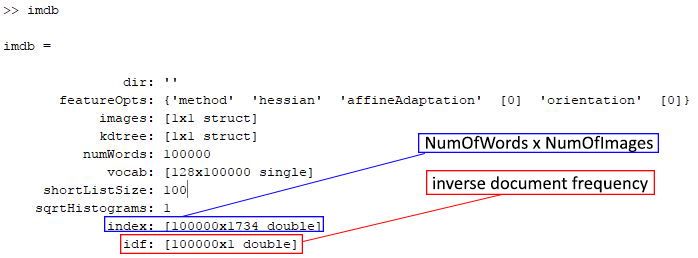
\includegraphics[scale=0.6]{imdb.jpg}
  \caption{image database structure}
\end{figure}

\paragraph{}\textbf{2.} the image database takes $\mathcal{O}(NumOfWords \times NumOfImages)$ Memory. \newline
Here we have: \textbf{NumOfWords} = 100000 and \textbf{NumOfImages} = 1734.

\paragraph{}\textbf{3.}
Stage of the search:
\begin{itemize}
\item We compute the histogram of the visual words in the query image and in the database images
\item We score each image of the database using an inverted file index. This can be done quite efficiently using Matlab's built-in sparse matrix engine.
\item We re-score the top-ranked images from the previous step using a geometric verifications step.
\end{itemize}

\begin{table}[H]
\centering
\caption{Search Times (in second) for each mystery images}
\label{Images recognition}
\begin{tabular}{llll}
\rowcolor[HTML]{EFEFEF} 
{\color[HTML]{000000} \textbf{Image}} & {\color[HTML]{000000} \textbf{The Starry Night}} & {\color[HTML]{000000} \textbf{Wheat Field with Cypresses}} & {\color[HTML]{000000} \textbf{Sedie}} \\
\textbf{Feature time} & 0.235 & 0.424 & 1.770 \\
\textbf{Index time} & 0.028 & 0.032 & 0.034 \\
\textbf{Geometric verification} & 0.372 & 0.541 & 1.967
\end{tabular}
\end{table}

\end{document}
